\documentclass{article}
\usepackage[utf8]{inputenc}
\usepackage[a4paper,top=2.5cm, bottom=3cm, outer=2.5cm, inner=2.5cm, heightrounded, marginparwidth=5cm, marginparsep=0.5cm]{geometry}
\usepackage[ngerman]{babel}
\usepackage{amsmath}
\usepackage{amsfonts}
\usepackage{amssymb}
\usepackage{graphicx,caption}
\usepackage{float}

\addto{\captionsngerman}{
  \renewcommand*{\contentsname}{Inhalt}
  \renewcommand*{\listfigurename}{Abbildungen}
  \renewcommand*{\listtablename}{Tabellen}
  \renewcommand*{\figurename}{Abbildung}
  \renewcommand*{\tablename}{Tabelle}
}

\setlength\parindent{0pt}
\DeclareCaptionFormat{myformat}{\fontsize{7}{8}\selectfont#1#2#3}
\captionsetup{format=myformat}


\begin{document}
\section{Zielsetzung}
In folgender Aufgabe ist es unser Ziel mit Hilfe von Wärmebildaufnahmen der "Seek Thermal" Anwendung den Emissionsgrad zweier Flächen des "Leslie" Würfels zu bestimmen.
Hierzu werden zwei verschiedene Datenquellen herangezogen: einerseits das Wärmebild im JPEG Format, andererseits die unveränderten Temperaturwerte aus einer TIFF Datei.
Beide Quellen repräsentieren jeweils dieselbe Aufnahme, wodurch ein direkter Vergleich möglich ist.
In unserer Vorgehensweise zur Auswertung legen wir besonderen Wert auf die Quantifizierung der Messunsicherheit diverser Quellen.
Neben der Möglichkeit die statistische Signifikanz der Ergebnisse zu evaluieren, lässt sich so besser Abschätzen, ob zusätzliche Fehlerfaktoren unzureichend berücksichtigt wurden.

\section{Auswertungsmethodik}
\subsection{JPEG Verarbeitung}
Die Aufnahmen der Kamera werden von der Software standardmäßig als JPEG Dateien abgespeichert.
Dies ist für eine weitere quantitative Auswertung problematisch, da die gemessenen Temperaturen in RGB-Werte umgewandelt werden.
Zusätzlich ist die Erstellung von JPEG Dateien mit dem Verlust von Bildinformation gekoppelt. 
Dementsprechend ist es für eine quantitative Auswertung notwendig die ursprünglichen Temperaturinformationen für jeden Pixel möglichst genau wiederherzustellen.
Dies wird in zwei Schritten bewerkstelligt:
Einerseits der Zuordnung von Farb- und Temperaturwerten mittels des im Bild inkludierten Farbbalkens, andererseits der Umwandlung aller Pixel in Temperaturen.

\subsubsection{Farb-Temperatur Zuordnung}

Jedes Bild verfügt über eine Farbskala, welche zum visuellen Abschätzen der Temperaturen innerhalb des Bildes dient.
Bei der Wahl des Aufnahmemodus ist es wichtig eine lineare Farbskala zu verwenden, da es andernfalls nicht möglich ist eine genaue Temperaturzuordnung zu finden.
Der Maximal- und Minimalwert der Skala ist in der App jeweils mit der entsprechenden Temperatur gekennzeichnet.
Mit Hilfe dieser Informationen lässt sich eine Zuordnung von Farbwert und Temperatur erzeugen.
Für den $k$-ten Pixel des Farbskala kann die korrespondierende Temperatur $T_{k}$ mittels folgender Formel berechnet werden:

\begin{equation}
    T_{k} = \frac{k}{n} \left(T_{max} - T_{min}\right) + T_{min}
\end{equation}

wobei $n$ die Anzahl der Pixel der Farbskala repräsentiert.
Die beiden angegebenen Randtemperaturen $T_{min}$ und $T_{max}$ werden jeweils ganzzahlig angezeigt.
Dies lässt die Frage offen, ob diese zur Präsentation auf- oder abgerundet wurden.
Die Standardunsicherheit der Randtemperaturen $u_{round}$ kann quantifiziert werden durch:

\begin{equation}
    u_{round} = \frac{0.5}{\sqrt{3}}
\end{equation}

Folglich ergibt sich ein möglicher Temperaturfehler für jeden Farbwert der Skala, welcher sich über die Fehlerfortpflanzung berechnen lässt:

\begin{equation}
    u_k = \sqrt{\left(\frac{k}{n} u_{round} \right)^2 + \left(\left(1 - \frac{k}{n}\right) u_{round}\right)^2}
\end{equation}

Hier beschreibt $u_k$ die Standardunsicherheit des berechneten Temperaturwerts der $k$-ten Skalenfarbe.

\subsubsection{Farbinterpolation}
Nun sind zwar die Temperaturen für alle Farben der Farbskala bekannt, jedoch können die Pixel des eigentlichen Bildes Farbwerte besitzen, die zwischen jenen der Skala liegen.
Mit Hilfe von Interpolation lassen sich auch diesen Farben Temperaturen zuordnen.
Im Allgemeinen ist die Interpolation von RGB Werten jedoch keine einfache Aufgabe. 
Der Farbverlauf der Skala stellt eine dreidimensionale Kurve im RGB-Raum dar, welche auf Grund des JPEG Formats über ungenaue Farbwerte verfügt.
Dies schließt die Anwendung vieler üblicher Interpolationsmethoden aus.
Eine mögliche Variante ist der Einsatz von Nearest-Neighbor Interpolation, welche allerdings zu einem zusätzlichen Interpolationsfehler führt.
\\
\\
Alternativ kann durch die Verwendung einer Skala in Graustufen das Problem der Farbinterpolation im Gesamten umgangen werden.
In diesem Fall liegen alle Farbwerte auf einer eindeutig definierten Linie, wodurch lineare Interpolation ein präzises Ergebnis liefert.

\begin{figure}[H]
    \centering
    \captionsetup{width=8cm}
    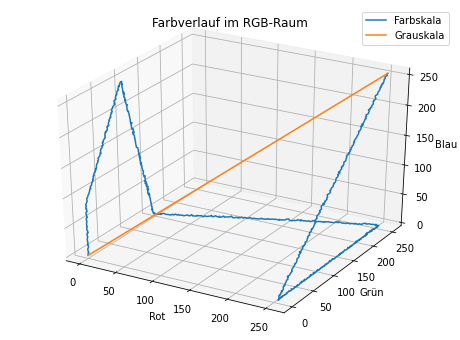
\includegraphics[width=10cm]{img/farb_vs_grau.png}
    \caption{Vergleich der Kurve einer Farbskala und einer Grauskala im RGB-Raum.}
\end{figure}

Die zugehörigen Unsicherheitswerte der Temperatur für jeden Pixel im Bildes $u_i$ können ebenso interpoliert werden.
Sie kombinieren sich mit der thermischen Messungenauigkeit der Kamera.
Eine Internetrecherche hat für das Modell "Seek Compact XR" eine Temperaturtoleranz von $tol_{th} = 0.07 ^{\circ}C$ ergeben.
Weitere Informationen konnten nicht aufgefunden werden.

\begin{equation}
    u_{th} = \frac{tol_{th}}{\sqrt{3}}
\end{equation}

\begin{equation}
   u_i = \sqrt{ u_{th}^2 + u_{k,interp}^2 } 
\end{equation}

\subsection{TIFF Verarbeitung}
Die Wahl der entsprechenden Einstellung in der Seek Thermal App ermöglicht es aufgenommene Bilder im TIFF Format abzuspeichern. 
Dieses Bildformat ist in der Lage mehrere Bilder in eine Datei zusammenzufassen.
Im Falle der Seek App befinden sich darunter auch die gemessenen unveränderten Temperaturwerte.
Dementsprechend entfällt die Notwendigkeit die Temperaturen von den Farbwerten der Pixel abzuleiten.
Der relative Fehler jedes Temperaturwertes ist in diesem Fall rein von der thermischen Messgenauigkeit der Kamera bestimmt.

\subsection{Emissionsgradbestimmung}
Im Falle eines schwarzen Körpers ist die von der Kamera erfasste Strahlungsleistung definiert durch:

\begin{equation}
    P(T) = \sigma f T^4
\end{equation}

Die reale erfasste Strahlungsleistung kann vereinfacht mittels des Emissionsgrades ausgedrückt werden. 
Der Anteil der reflektierten Strahlung wird während der Versuche als konstant angenommen.
Dementsprechend kann aus der Differenz zwischen der gemessenen Temperatur $T_m$ und tatsächlichen Temperatur $T_w$ aus zwei Versuchen der Emissionsgrad $\epsilon$ berechnet werden.

\begin{equation}
    P(T_m) = \epsilon \cdot P(T_w) + (1 - \epsilon) \cdot P(T_u)
\end{equation}
 
\begin{equation}
   T_m^4 = \epsilon \cdot T_w^4 + (1 - \epsilon) \cdot T_u^4
\end{equation}

\begin{equation}
    T_m^4 - \epsilon \cdot T_w^4 = (1 - \epsilon) \cdot T_u^4 = C = \textit{const.}
\end{equation}

\begin{equation}
    T_{m,1}^4 - \epsilon \cdot T_{w,1}^4 = T_{m,2}^4 - \epsilon \cdot T_{w,2}^4 
\end{equation}

\begin{equation}
    \epsilon = \frac{T_{m,1}^4 - T_{m,2}^4}{T_{w,1}^4 - T_{w,2}^4}
\end{equation}

Um die Genauigkeit des auf diese Weise bestimmten Emissionsgrades zu erhöhen, werden an Stelle eines einzelnen gemessenen Temperaturwertes $T_m$ die gemittelten Temperaturen $\overline T_m$ innerhalb eines definierten Refernzbereiches verwendet.

\begin{equation}
    \overline T_m = \frac{1}{n} \sum_{i=1}^n T_i
\end{equation}

Da der Emissionsgrad der Referenzstelle ($\epsilon_{w}$) bekannt ist, kann der Emissionsgrad der Kamera ($\epsilon_{m}$) berechnet werden.
Weiters kann für das gesamte Bild der Emissionsgrad jedes einzelnen Pixel bestimmt werden.
Diese Werte beziehen sich auf die tatsächliche Temperatur des Körpers $T_w$ und sind nur für diesen gültig.

\begin{equation}
    \epsilon_{m} = \frac{\epsilon}{\epsilon_{w}}
\end{equation}

\begin{equation}
    \epsilon_i = \frac{T_i^4 - C}{\epsilon_{m} \cdot T_w^4}
\end{equation}

Die entsprechenden Standardunsicherheiten können mit folgenden Formeln berechnet werden:

\begin{equation}
    u_{\overline T_m} = \sqrt{ \sum_{i=1}^n \left( \frac{u_{T_i}}{n} \right)^2 }
\end{equation}

\begin{equation}
    \frac{\partial \epsilon}{\partial T_{m,1}} = \frac{4T_{m,1}^3}{T_{w,1}^4 - T_{w,2}^4} 
\end{equation}

\begin{equation}
    \frac{\partial \epsilon}{\partial T_{m,2}} = -\frac{4T_{m,2}^3}{T_{w,1}^4 - T_{w,2}^4}
\end{equation}

\begin{equation}
    \frac{\partial \epsilon}{\partial T_{w,1}} = -\frac{4T_{w,1}^3 \left( T_{m,1}^4 - T_{m,2}^4 \right)}{\left( T_{w,1}^4 - T_{w,2}^4\right)^2} 
\end{equation}

\begin{equation}
    \frac{\partial \epsilon}{\partial T_{w,2}} =  \frac{4T_{w,2}^3 \left( T_{m,1}^4 - T_{m,2}^4 \right)}{\left( T_{w,1}^4 - T_{w,2}^4 \right)^2}
\end{equation}

\begin{equation}
    u_\epsilon = \sqrt{
        \left( \frac{\partial \epsilon}{\partial T_{m,1}} \right)^2 u_{T_{m,1}}^2 + 
        \left( \frac{\partial \epsilon}{\partial T_{m,2}} \right)^2 u_{T_{m,2}}^2 + 
        \left( \frac{\partial \epsilon}{\partial T_{w,1}} \right)^2 u_{T_{w,1}}^2 + 
        \left( \frac{\partial \epsilon}{\partial T_{w,2}} \right)^2 u_{T_{w,2}}^2
    }
\end{equation}

\begin{equation}
    u_C = \sqrt{\left( 4 T_m^3 \right)^2 u_{T_m}^2 + \left( -4 \epsilon T_w^3 \right)^2 u_{T_w}^2 + \left( -T_w^4 \right)^2  u_{\epsilon}^2} 
\end{equation}

\begin{equation}
    u_{\epsilon_m} = \sqrt{ \left( \frac{1}{\epsilon_w} \right)^2 u_\epsilon^2 + \left( -\frac{\epsilon}{\epsilon_w^2} \right)^2 u_{\epsilon_w}^2}
\end{equation}

\begin{equation}
    u_{\epsilon_i} = \sqrt{ 
        \left( \frac{4 T_i^3}{\epsilon_m T_w^4} \right)^2 u_{T_i}^2 + 
        \left( -\frac{1}{\epsilon_m T_w^4} \right)^2 u_C^2 +
        \left( -\frac{T_w^4 \left( T_i^4 - C \right) }{\left( \epsilon_m T_w^4 \right)^2} \right)^2 u_{\epsilon_m}^2 +
        \left( -\frac{4 \epsilon_m T_w^3 \left( T_i^4 - C \right)}{\left( \epsilon_m T_w^4 \right)^2} \right)^2 u_{T_w}^2
      }
\end{equation}

\subsection{Annahmen der Fehlerbereiche}
In folgender Tabelle sind unsere Abschätzungen der Toleranzbereiche angeführt:

\begin{center}
    \begin{tabular}{llll}
        Name & betreffende Variable(n) & Fehlerbereich & zugehörige Standardunsicherheit\\
        \hline
        Thermische Auflösung & $T_i$ & $\pm 0.07 ^{\circ}C$ & $u_{th}$\\
        Skalenrundung & $T_\textit{min},\ T_\textit{max}$ & $\pm 0.5 ^{\circ}C$ & $u_{round}$\\
        Referenztemperatur & $T_{w,1},\ T_{w, 2}$ & $\pm 0.5 ^{\circ}C$ & $u_{T_w}$\\
        Referenzemissionsgrad & $\epsilon_w$ & $\pm 0.05$ & $u_{\epsilon_w}$\\
        \hline
    \end{tabular}
\end{center}

\section{Ergebnisauswertung}
Das zuvor beschriebene Verfahren kann nun verwendet werden, um die Emissionsgrade der Flächen des Leslie Würfels abzuschätzen.
Im ersten Schritt werden die Werte bei Verwendung der selben Kalibrierungsaufnahmen verglichen.


\begin{figure}[H]
    \centering
    \captionsetup{width=12cm}
    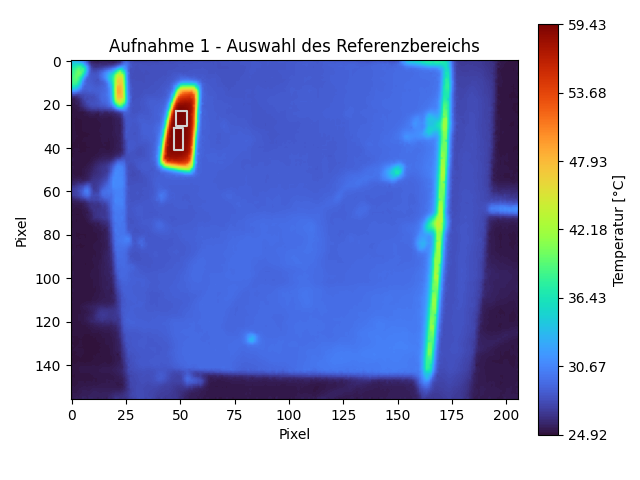
\includegraphics[width=6cm]{img/ref_sel_1.png}
    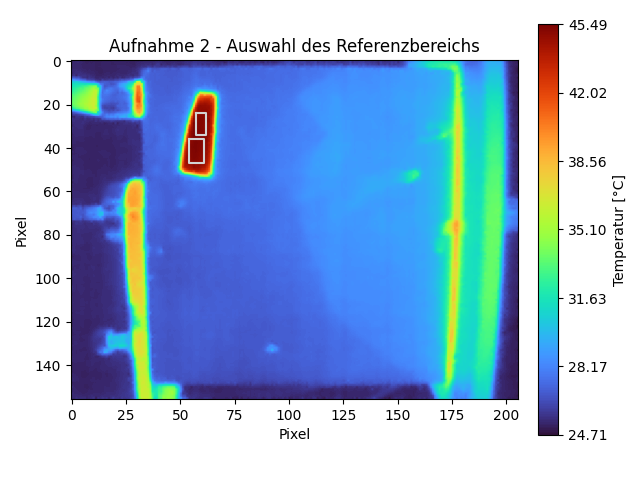
\includegraphics[width=6cm]{img/ref_sel_2.png}
    \caption{
        Die Auswahl eines Referenzbereiches (graue Rechtecke) mit bekanntem Emissionsgrad für beide Bilder.
        Aus diesem Bereich werden alle Temperaturwerte zur Berechnung des tatsächlichen Emissionsgrades gemittelt. 
    }
\end{figure}

\begin{figure}[H]
    \centering
    \captionsetup{width=12cm}
    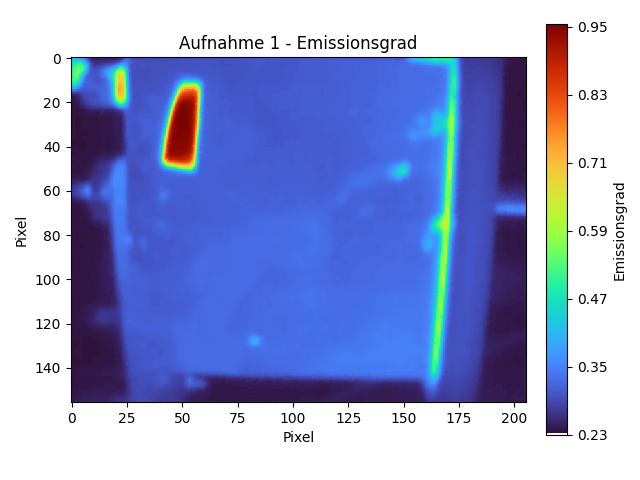
\includegraphics[width=6cm]{img/eps_1.png}
    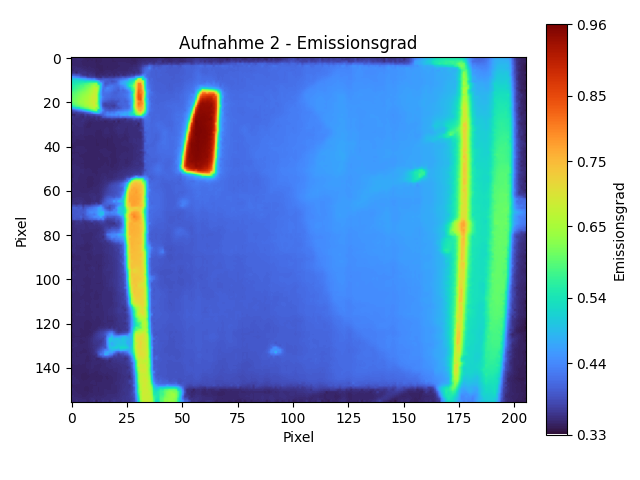
\includegraphics[width=6cm]{img/eps_2.png}
    \caption{
        Der berechnete Emissionsgrad für jeden Pixel der beiden Bilder.
        Da die Temperatur des Würfels als Referenz herangezogen wurde, ist das Resultat nur für diesen gültig.
    }
\end{figure}

\section{Schlussfolgerung}

\end{document}